\section{Program partition and proof batching}
\label{chp:sharding-batching}
As discussed in Section \ref{chp:foreign}, when encoding execution trace in $T_\mathcal{E}$, each instruction will take a constant number of rows. In Halo2 proof system, there is a limit of the total number of rows of arithmetic circuits \cite{halo2book}. Therefore, for large WASM images, we probably can not fit the whole execution trace into $T_\mathcal{E}$. To solve the problem of long execution trace,  \zkwasm\, use the technique of program partition and proof batching. The idea is that we split the execution trace $\left[t_0,t_1,\cdots\right]$ into group of sub sequences, generate execution proof for each group and batch all the proofs in the end. Here we first give a bold sketch about the overview of the technique and then presents the extra constraints we need to provide when batching sub proofs.

\smallskip Given an execution sequence $t_i$, we split it into small execution chunks $t_{[a,b]} = {t_a, t_{a+1}, \cdots, t_{b-1}}$ and denote the $\mathcal{M}_{[a,b]}, \mathcal{SP}_{[a,b]}$, $\mathcal{G}_{[a,b]}$ to be the memory, stack and global access log related to $t_{[a,b]}$. We notice that given a execution trace $t_{[a,b]}$, by using the arithmetic circuits constructed in Section \ref{chp:architecture-circuits}, we can prove $t_{[a,b]}$ is valid under the context \partialstate{a}{b}. We denote $\mathcal{P}_{[a,b]}$ the proof of the valid execution of $t_{[a,b]}$ and $\mathcal{P}$ is the proof of the valid execution of $t_i$ under the full access log \fullstate. Now it remains to find out what conditions we need to enforce so that
\[
   (\mathcal{P}_{[0,k-1]} \wedge   \mathcal{P}_{[k,2k-1]} \wedge \cdots \wedge   \mathcal{P}_{[0,end]}) \rightarrow
     \mathcal{P}.
\]
\noindent Thus it is sufficient to make sure that for each $t_i \in t_{[a,b]}$ the constraints applied on it in $\mathcal{P}_{[a,b]}$ is equivalent to the constraints applied on it in $\mathcal{P}$. As we have presented in Section \ref{chp:architecture-circuits}, constraints applied on each instruction block in $T_\mathcal{E}$ contains two parts, that are polynomial constraints about cells of the current and next instruction block and constraints of polynomial lookup of state (memory, stack, global) access logs.\\

\noindent\emph{Equivalent of Polynomial Constraints.} Regarding the polynomial constraints of cells, it is easy to check that if $t_i\in t_{[a,b]}$ and $i<b$ then all polynomial constraints of cells of the instruction block of $t_i$ in $\mathcal{P}_{[a,b]}$ are equal to the those in $\mathcal{P}$. So it remains to constraint that the last instruction of $t_{[a,b]}$ has the same polynomial constraints both in $\mathcal{P}_{[a,b]}$ and $\mathcal{P}$. However, it is not true in general since if we split the execution sequence into blocks that are disjoint, then the connection between two sequences are lost. Therefore, to solve this problem, we need to pad a glue instruction at the end of each sub sequence and enforce the address of the glue instruction equal to the address of the first instruction of next block (see Figure \ref{fig:subsequence}). By doing so we can check that the polynomial constraints of each $t_i$ in $\mathcal{P}_{[a,b]}$ is equivalent as it is in $\mathcal{P}$. \\

\begin{figure}[!ht]
\centerline{
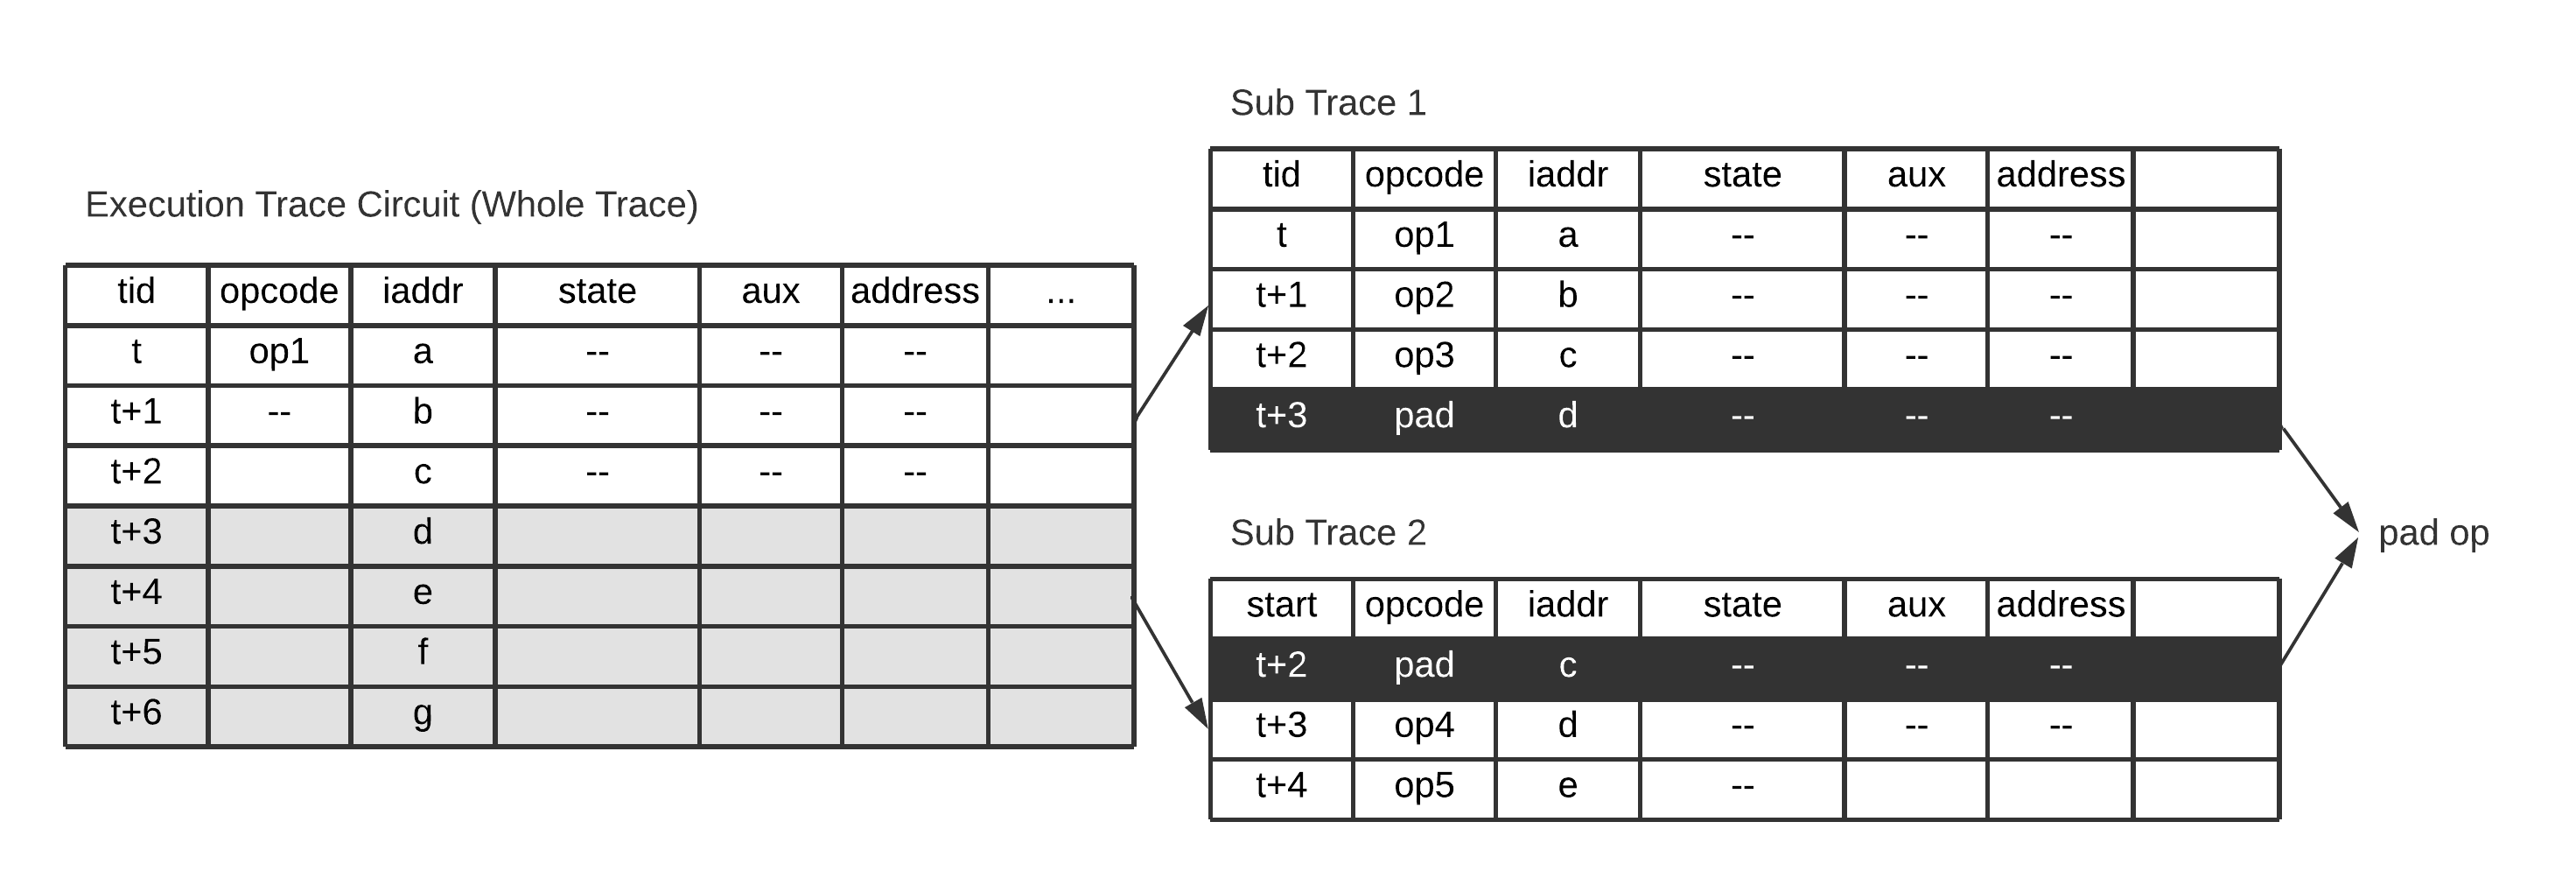
\includegraphics[scale=0.6]{figs/subsequence.png}
}
\caption{Split execution sequence into sub sequence}
\label{fig:subsequence}
\end{figure}

\noindent\emph{Equivalent of Polynomial Lookup.} Given a constraint of polynomial lookup for a cell in $t_i$, we need to show that $c \in \mathbf{T}_\mathcal{M}$ if and only if $c \in \cup \mathbf{T}_{\mathcal{M}_{k}}$. By the definition of Equation \ref{eq:rw-constraints} we know that the property hold if and only if the concatenate of $\mathbf{T}_{\mathcal{M}_k}$ satisfies Equation \ref{eq:rw-constraints}. Notice that Equation \ref{eq:rw-constraints} only constraints adjacent rows, we extract a glue table $\mathbf{TG}_\mathcal{M}$ for $\mathbf{T}_{\mathcal{M}_{k}}$ ($k = 1,2,\cdots$) as in (Figure \ref{fig:tbl-glue}) and then it follows that $\mathbf{T}_\mathcal{M} = \cup \mathbf{T}_{\mathcal{M}_{k}}$ if $\mathbf{T}_\mathcal{M}$, $\mathbf{T}_{\mathcal{M}_{k}}$ and $\mathbf{TG}_\mathcal{M}$ all satisfy Equation \ref{eq:rw-constraints}.

\begin{figure}[!ht]
\centerline{
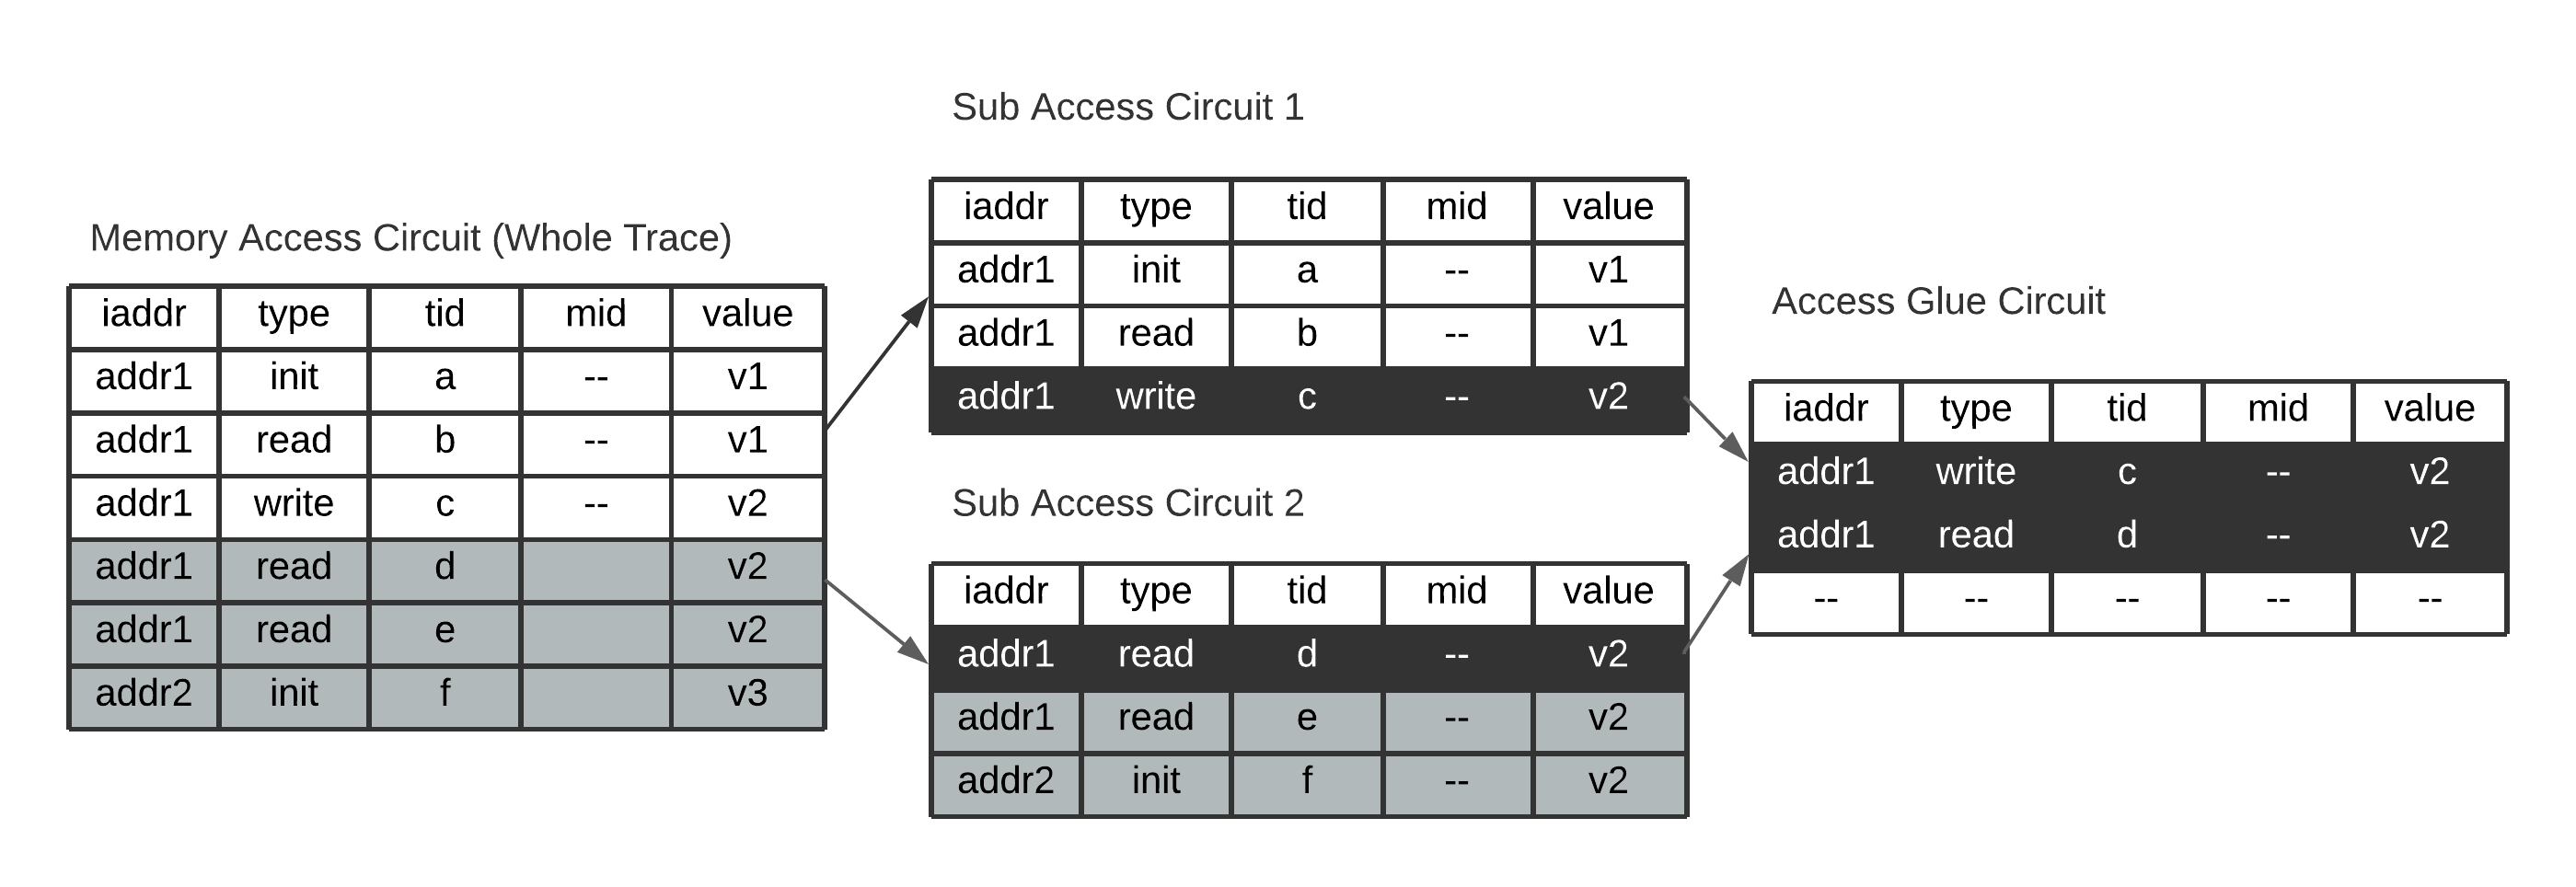
\includegraphics[scale=0.6]{figs/memory-glue.png}
}
\caption{Split memory access log into sub log}
\label{fig:tbl-glue}
\end{figure}

\smallskip As a conclusion, to solve the long execution trace problem, we split the execution trace into $t_{[a_0,b_0]}, t_{[a_1,b_1]}, t_{[a_2, b_2]}, \cdots$ and construct $\mathbf{T}_{\mathcal{M}_{k}}$ $\mathbf{T}_{\mathcal{SP}_{k}}$ $\mathbf{T}_{\mathcal{G}_{k}}$ for execution block $t_{[a_k, b_k]}$. Suppose that $\mathcal{P}_k$ proves the valid execution of $t_{[a_k,b_k]}$ and $\mathbf{TG}_\mathcal{M}$ is the glue map constructed as in Figure \ref{fig:tbl-glue}, then we claim that a proof $\mathcal{P}_{batch}$ can prove that the execution sequence $t_i$ is a valid execution if and only if $\mathcal{P}_{batch}$ is the batched proof of all the constraints in Equation \ref{eq:split-eq}.
\begin{equation}
   \begin{cases}
        \mathcal{P}_k \textrm{ proves }  t_{[a_k,b_k]} \textrm{ is a valid execution under } (\mathcal{F}, \mathcal{M}_{[a_k,b_k]}, \mathcal{SP}_{[a_k,b_k]}, \mathcal{I}(\mathcal{C,\mathcal{H}})). \\
        t_{b_{k+1}}.iaddr = t_{a_{k}}.iadr \textrm{ when $k>0$ }. \\
        t_{b_{k}} \textrm{ is a glue instruction when $k>0$ and is not the last exectuion block}. \\
        TG_\mathcal{M} \textrm { satisfies Constraint \ref{eq:rw-constraints}}. \\
   \end{cases}
    \label{eq:split-eq}
\end{equation}

\noindent In \zkwasm, we write the verifying algorithm of $\mathcal{P}_k$ into arithmetic circuits $\mathcal{V}_k$ and the total batch circuit of Equation \ref{eq:split-eq} is construct by putting the verifying circuits together with the circuits that do the other simple checks.

\begin{remark}
Proof batching is an active research topic. Instead of writing verify function into arithmetic circuits, there are other methods \cite{ben2017scalable-batch,chiesa2019cycles-batch,habock2021darlin-batch,kothapalli2022nova-batch} that are worth trying as well. Since we are more focus on the consistency of program partition and memory access log in this paper, we leave the analyzing of trying different batching methods as future work.
\end{remark}